% !TEX root = ../gnss_interference_resistant_thesis.tex
\documentclass[main.tex]{subfiles}

\begin{document}

\subsection{Spindulio formavimas}

Spindulio formavimas (angl. Beamforming), arba erdvinis formavimas, yra radijo signalų apdorojimo
metodas,
naudojamas pasitelkiant antenų masyvus. Spindulio vairavimas pasiekiamas kombinuojant
signalus iš atskirų antenų sukuriant konstruktyvią interferenciją, taip sudarant
maksimumus.

\begin{figure}[h]
    \begin{centering}
    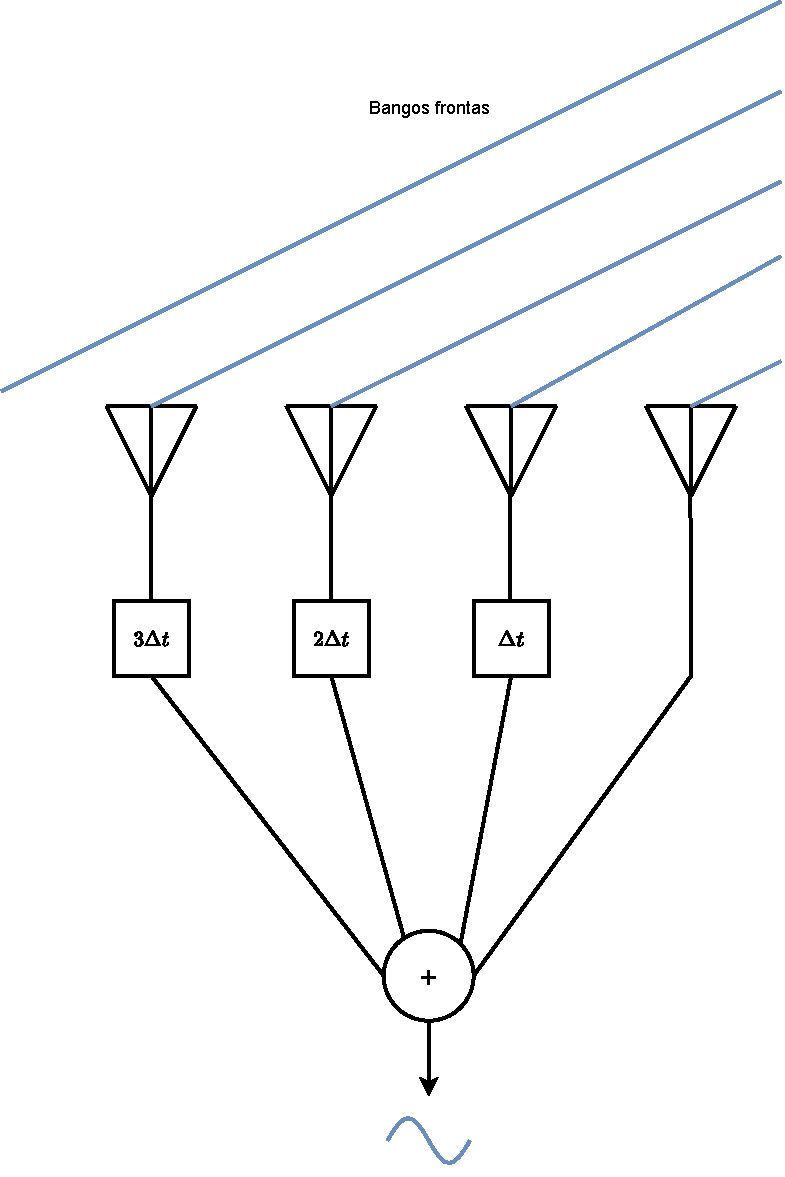
\includegraphics[scale=0.5]{drawings/simple_steering}
    \par\end{centering}
    \protect\caption{\label{fig:simple_steering}4 elementų masyvo spindulio formavimo schema.}
\end{figure}

Norint susidaryti supratimą, kaip veikia spindulio vairavimas, galima
pasinaudoti nesudėtinga iliustracija \ref{fig:simple_steering}~pav.
Paveiksliuke pavaizduota 4 elementų spindulio vairavimo sistema. Kiekvienam
RF signalui yra pritaikomas tam tikras užvėlinimas ($\Delta t$), parinkus
tinkamas vertes gaunama konstruktyvi interferencija tik signalui atėjusiam
iš pasirinktos krypties. Signalams atėjusiems iš kitos krypties, sumatoriuje
atėjusio signalo fazės nebeatitinka, todėl gaunama destruktyvi interferencija.
Keičiant signalo užlaikymą (fazę), galima gauti signalo maksimumą norima
kryptimi.

Pasinaudojus \ref{fig:beamform_path}~pav. schema, galima suskaičiuoti vėlinimo laiką ($\Delta t$), arba reikalingą
fazės pokytį ($\Delta\Phi$).

\begin{figure}[h]
    \begin{centering}
    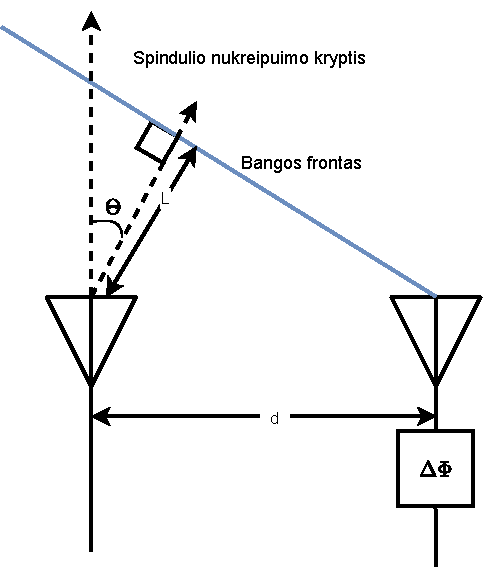
\includegraphics[scale=0.8]{drawings/beamform_path}
    \par\end{centering}
    \protect\caption{\label{fig:beamform_path}Bangos vėlinimui suskaičiuoti skirtas brėžinys.}
\end{figure}

Laiko vėlinimas:
\begin{equation}
    L = d\sin(\Theta),
\end{equation}
\begin{equation}
    \Delta t = \frac{L}{c}=\frac{d\sin(\Theta)}{c},\ c = 3 * 10^8\ \mathrm{m/s}.
\end{equation}
Žinant laiko vėlinimą, galime nesunkiai suskaičiuoti fazės pokytį:
\begin{equation}
    \Delta \Phi = \frac{2\pi c \Delta t}{\lambda} = \frac{2\pi d \sin{\Theta}}{\lambda}
    \label{eq:phase_shift}
\end{equation}
Laikant, kad $d = \lambda / 2$, \refeq{eq:phase_shift} lygtis supaprastėja ir gauname:
\begin{equation}
    \Delta \Phi = \pi \sin{\Theta}
    \label{eq:phase_shift_antenna_angle}
\end{equation}

Norint įvertinti spindulio formą, iš kelių antenų, galime įsivesti masyvo faktorių
$AF$ (angl. array factor). Šis parametras nurodo spindulio formą, neatsižvelgus
į antenų, sudarančių masyvą, spindulio formą. Turint antenos spindulio formą
ir $AF$, antenų masyvo spindulio forma galime gauti sudėjus abu parametrus
(jeigu jie yra išreikšti $\mathrm{dB}$ vienetais).
$AF$ išraiška N-antenų masyvui, kai jos yra vienoje plokštumoje \cite{phase_array_handbook}:
\begin{equation}
    AF(\Theta,\Delta \Phi) = \frac{\sin{\left( N\left[ \frac{\pi d}{\lambda} \sin{\Theta} - \frac{\Delta \Phi}{2} \right] \right)}}{N \sin{\left( \frac{\pi d}{\lambda}\sin{\Theta}-\frac{\Delta \Phi}{2}\right)}}
    \label{eq:array_factor}
\end{equation}
Pasinaudojus \refeq{eq:array_factor} lygtimi galime nubraižyti spindulio formą (\ref{fig:af_polar_plot}~pav.), kai $d=\lambda /2$.

\begin{figure}[h]
    \begin{centering}
    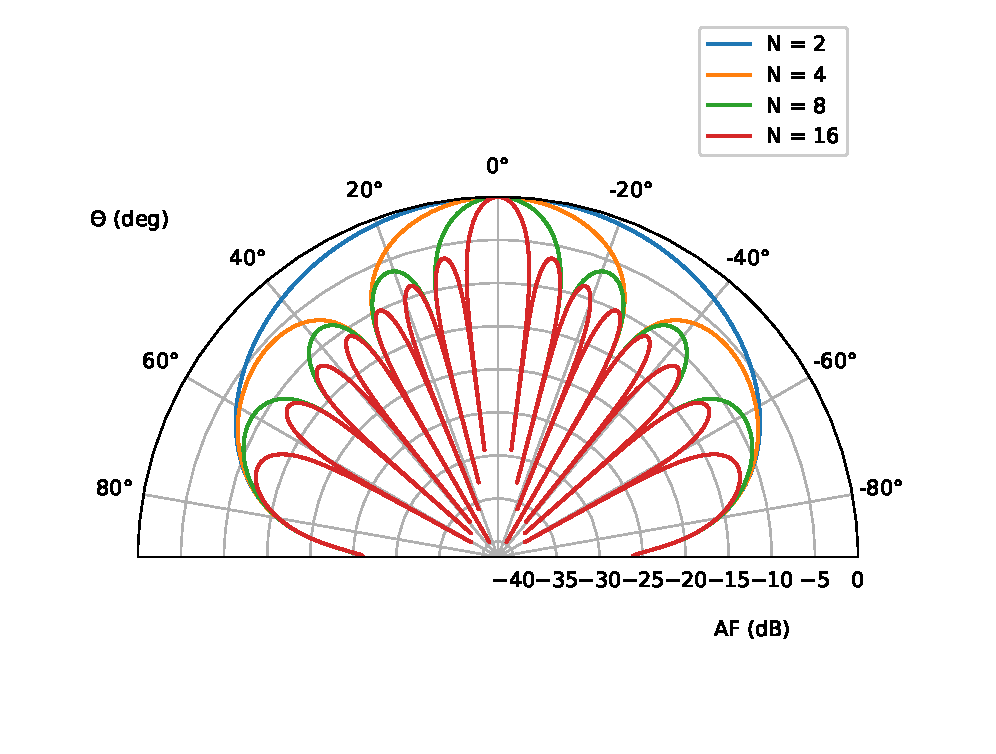
\includegraphics[scale=0.8]{drawings/af_polar_plot}
    \par\end{centering}
    \protect\caption{\label{fig:af_polar_plot}AF esant skirtingam skaičiui antenų masyve, kai $d=\lambda / 2$ ir $\Delta \Phi = 0$.}
\end{figure}


\end{document}
